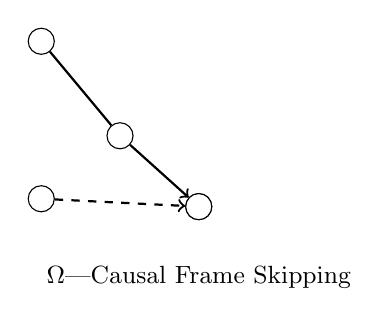
\begin{tikzpicture}[
    node/.style={circle,draw=black,fill=white,minimum size=5pt},
    arrow/.style={->, thick}
]

\node[node] (A1) at (-2,1) {};
\node[node] (A2) at (-1,-0.2) {};
\node[node] (A3) at (0,-1.1) {};

\node[node] (B1) at (-2,-1) {};
\node[node] (B3) at (0,-1.1) {};

\draw[arrow] (A1)--(A2)--(A3);
\draw[arrow,dashed] (B1)--(B3);

\node at (0,-2) {\small $\Omega$---Causal Frame Skipping};

\end{tikzpicture}